\begin{answer}

If you just care about the case reflected by implementation in (b), with the same naive stop condition, you can just look at node number from 0 to 4 
\begin{figure}[H]
    \centering
    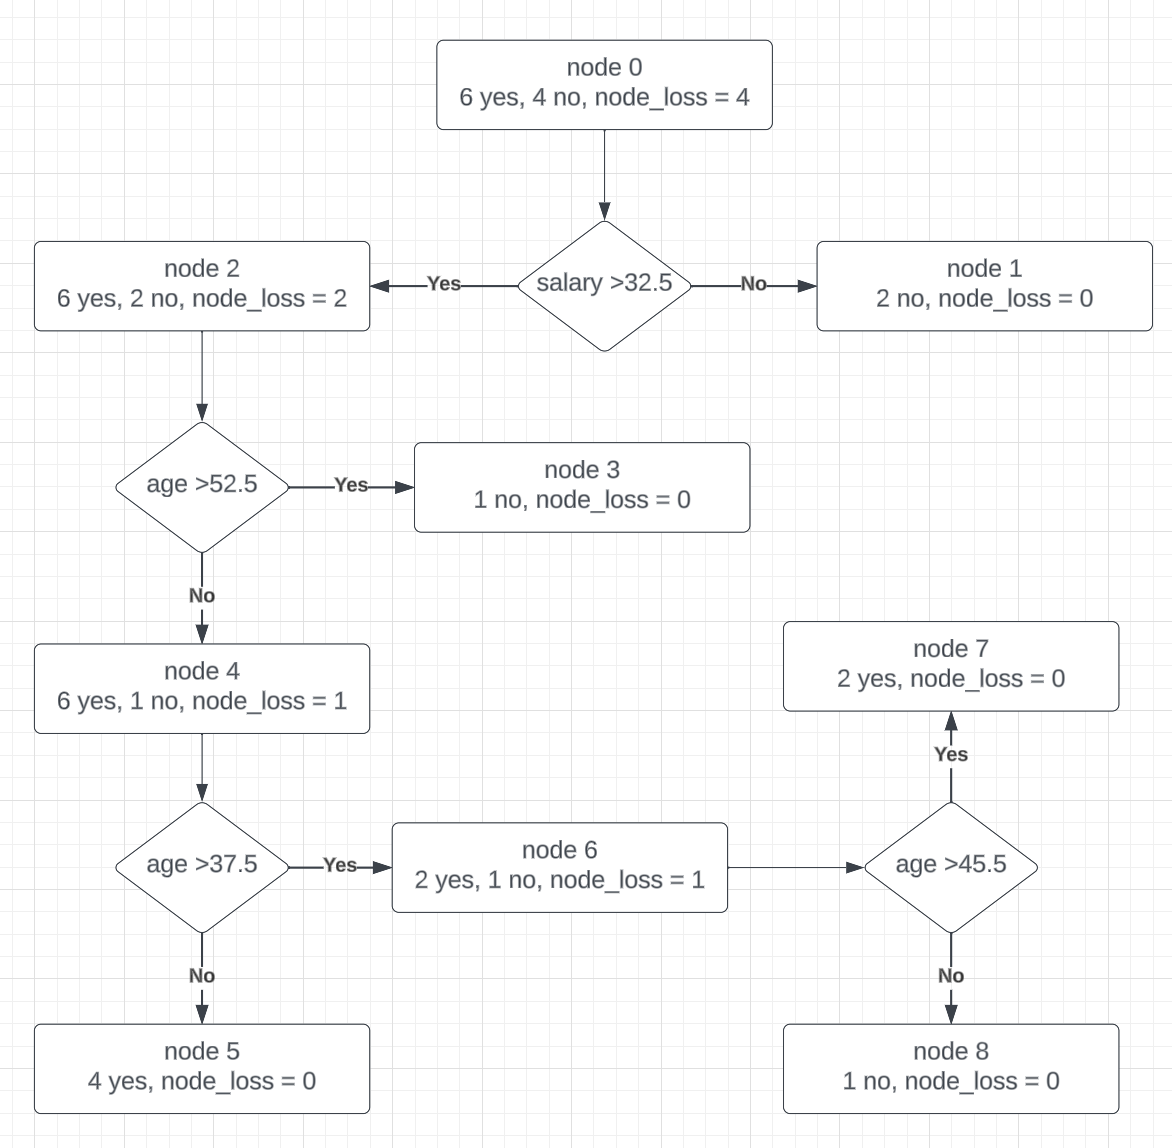
\includegraphics[width=0.5\linewidth]{Screenshot 2024-02-20 at 21.17.01.png}
    \caption{ps3::q1::a}
    \label{fig:enter-label}
\end{figure}
% depth 0, root node 0, split by salary with threshold = 32.5, with loss = 2 \\
% depth 1, node 1, parent is node 0.  No split, and no loss.  \\
% depth 1, node 2, parent is node 0.  Split by age with threshold = 52.5, with loss = 1 \\
% depth 2, node 3, parent is node 2.  Split by age with threshold = 23, with loss = 1 \\
% depth 2, node 4, parent is node 2.  No split, and no loss. \\
\end{answer}